\documentclass[10pt]{article}
\usepackage[margin=.68in]{geometry}
\usepackage{graphicx,booktabs,hyperref,amsmath,amssymb,array}
\hypersetup{colorlinks=true,urlcolor=blue}
\setlength{\parindent}{0pt}
\setlength{\parskip}{5pt}
\newcommand{\study}{\texttt{quadratic\_twist\_evidence\_20261021}}
\begin{document}
\begin{center}
{\Large Mixed quadratic-twist relations: finite falsification}\\[4pt]
{\large An explicit Frobenius image bridge, checked in Lean}\\[4pt]
22 October 2026 $\cdot$ \texttt{mixed-20261022T0718Z} $\cdot$ PR \#2381
\end{center}
\textbf{Observed outcome.} Two native implementations agree on 74,693,760
ordered signed words on 274 odd-prime subgroup pairs. Every mixed zero relation
vanishes separately in the two Frobenius components. Mixed rows add no rank
over pure rows at the same maximum length. This rejects the specified finite
relation shortcut; it is not a general no-advantage or ECDLP hardness theorem.

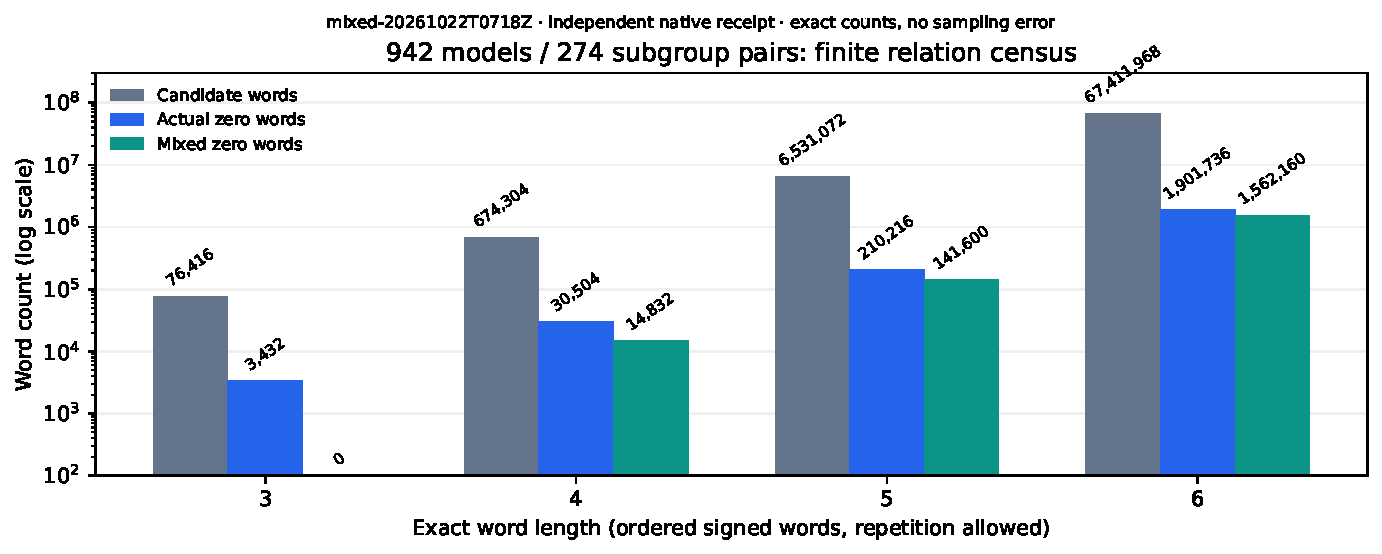
\includegraphics[width=\linewidth]{word-counts.pdf}
\small Exact counts from \texttt{native/mixed-20261022T0718Z/audit.json}.
The count axis is logarithmic; the zero at length three is explicit. Exhaustive
population, no sampling interval. Counts include repeated and dependent words;
they are not counts of independent information.\normalsize

\begin{center}\small
\begin{tabular}{rrrrr}
\toprule
Length & Candidates & Zero words & Mixed zero words & Mixed zero rows\\\midrule
3 & 76,416 & 3,432 & 0 & 0\\
4 & 674,304 & 30,504 & 14,832 & 14,832\\
5 & 6,531,072 & 210,216 & 141,600 & 0\\
6 & 67,411,968 & 1,901,736 & 1,562,160 & 637,200\\\bottomrule
\end{tabular}\normalsize\end{center}
Here ``mixed zero rows'' counts literally zero integer coefficient vectors;
other rows can also vanish modulo $r$. Nonzero integer mixed rows at
lengths five and six still supply no rank gain: their component relations are
already in the pure spans. All 1,096 subgroup/length comparisons pass.

\textbf{Frozen scope.} All 942 nonsingular short models with
$p\in\{5,7,11,13,17,19\}$ and $0\leq a,b<p$; least positive nonsquare $d$;
$K=\mathbb F_p[u]/(u^2-d)$. The run contains 186 cases at $r=3$, 72 at $r=5$,
and 16 at $r=7$. Every nonzero point of both selected cyclic subgroups is in
the alphabet, with signed representatives $1\leq j\leq(r-1)/2$. All points
are valid. This is the existing 942-model study, separate from the 4,493-model
global catalog. Existing ICV1 identities and exact generators are in each record.

\textbf{Method.} C++ reuses the native field/curve backend and exhausts ordered
words, verifying every accepted word by point addition and an injective
$r^2$ subgroup table. Independent Rust tuple arithmetic uses exponent inversion,
q-power Frobenius, forward Gaussian elimination and a coefficient-row dynamic
program with multiplicities. It decides all DP states by actual point addition.
This is same-host independent arithmetic/enumeration, with JSON/SHA and IDC1 shared.

\newpage
\begin{center}{\Large What is now proved, and what remains open}\end{center}
\textbf{Actual map.} Let $k$ be a finite field of odd characteristic, $d$ a
nonsquare, $K/k$ a field algebra containing $u^2=d$, and
$E:y^2=x^3+ax+b$ an elliptic short model. For the actual nonsingular points of
$E_d:Y^2=X^3+d^2aX+d^3b$, define
\[
\psi(O)=O,\qquad \psi(X,Y)=\left(\frac Xd,\frac Y{du}\right)\in E(K).
\]
Lean checks the target equation and injectivity. Nonzero denominators follow
from the nonsquare and field hypotheses. If $q=\#k$, Euler's criterion gives
\[
d^{(q-1)/2}=-1,\qquad u^q=u(u^2)^{(q-1)/2}=-u.
\]
Frobenius therefore fixes the x-coordinate of $\psi(P)$ and negates its
y-coordinate. This includes $O$ and derives the earlier \texttt{hB} assumption
for this explicit short-model image.

\textbf{Obstruction.} If rational lifts satisfy $A+\psi(P)=R$, applying
Frobenius gives $A-\psi(P)=R$, hence $2\psi(P)=O$. If also
$r\psi(P)=O$ with $\gcd(2,r)=1$, the image is zero and injectivity gives $P=O$.
Frobenius preserves addition, so the same obstruction applies to any finite
sum of explicit images with an odd annihilator. It kills the aggregate, not
every summand individually.

\begin{center}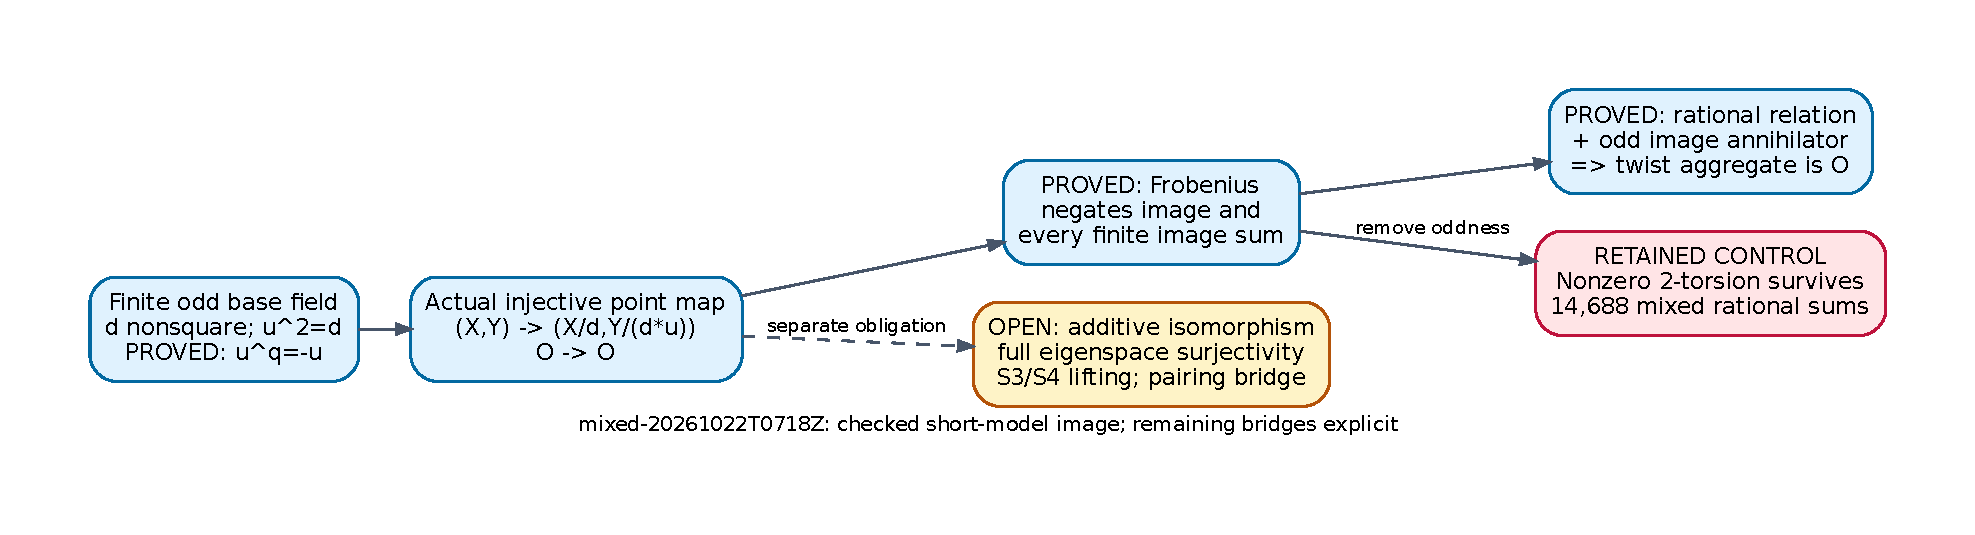
\includegraphics[width=\linewidth]{bridge.pdf}\end{center}

\textbf{Checked scope.} Ten new declarations bring the project to 28 named
research theorems. The final repository gate audits 36 declarations including
eight generated helpers, with zero failures and zero trusted native proofs.
Only \texttt{propext}, \texttt{Classical.choice}, and \texttt{Quot.sound} occur.
Lean 4.34.1 and Mathlib \texttt{d13f23b723b8a846827a245b89c10fc7d3f11612}
are pinned. The proof map is \path{lean/README.md}; the final source is
\path{lean/TwistEmbedding.lean}.

The universal cleared polynomial identity has certificate
\texttt{IDC1h9dc35b198cc2fa02}, bound to the exact final Lean source.
Native checking uses 32 derived and 16 extra evaluation points and rejects
an added-one false identity; the universal ring proof is checked separately.

\textbf{Open obligations.} The point map has not yet been declared an additive
isomorphism. The odd annihilator is explicitly on the actual image or sum;
transport from the source group is not silently assumed. Full eigenspace
surjectivity, general-model normalization, exceptional S3/S4 lifting,
pairing nondegeneracy/reduction and universal trace-zero geometry remain open.
The existing pairing connection and finite IC recoveries survive this result.
General hardness, a general GHS algorithm and a speedup are not established.

\newpage
\begin{center}{\Large Controls, receipts, and reproducible next steps}\end{center}
\begin{center}\small
\begin{tabular}{p{2.45in}p{3.85in}}
\toprule
Control / check & Observed result\\\midrule
All rational/twist pairs & 260,064 checked; rational sum iff the twist image is killed by two.\\
Oddness removed & 14,688 nonzero two-torsion exceptions; actual witnesses on 606 models.\\
Square parameter, $d=u=1$ & Fixed and not negated on 939 models; three models have only two-torsion rational points, explicitly null.\\
Identify scalar labels $P-T=O$ & Rejected by actual addition in all 274 odd-prime cases.\\
Corrupt a saved coefficient & Rejected as a nonzero actual curve sum, exit 101.\\
Delete one model & Rejected as missing coverage, exit 101; no replay receipt emitted.\\
Independent native replay & Full counts, signed rows, ranks and byte comparisons pass.\\
Proof gate & 36 declarations, zero failing, zero trusted native axioms.\\
Fresh library suite & 4,479 passed, 119 existing ignores, zero failures.\\
Isolated auditor backend tests & 22 passed, zero failures.\\
Shared Conductor & CLI unavailable, exit 127; no reservation or substitute coordinator.\\\bottomrule
\end{tabular}\normalsize\end{center}

\textbf{Preservation and failures.} The protocol was committed as
\texttt{6aa9212b4} before execution, on PR head \texttt{036c2a1a3292}.
Historical archives, earlier finite results, native snapshots and dated reports
remain unchanged. Catalog provenance still requires both \texttt{a11984a57344}
and \texttt{228cdc0d50f2}. Initial oversized-registry parsing, Rust visibility,
Lean elaboration and a read-only cache-path failure are retained. A supported
writable Mathlib cache path fixes the local environment failure; no proof gate
was bypassed. Failed attempts are not mathematical counterexamples.

\textbf{Reproduce from the repository root.}
\begin{quote}\small\ttfamily
bash research/quadratic\_twist\_evidence\_20261021/run-mixed.sh /tmp/twist-mixed-fresh
\end{quote}
Run \path{tools/lean/proof-gate.sh} on the study's \path{lean/} directory
for the pinned proofs. The workflow now executes the mixed-word replay,
independent arithmetic/ranks, exact-byte checks and corruption controls.
Raw records: \path{native/mixed-20261022T0718Z/}.
Commands, input/source hashes, logs and exits:
\path{validation/mixed-20261022T0718Z/}.

\textbf{Accounting.} Uncontrolled Linux x86-64 managed workspace; GCC 14.2,
OpenSSL 3.5.7 and Rust 1.99.1. Native limits: 300 seconds per full invocation,
not hit. No admitted wall-time comparison or unknown-log solver benchmark.
Setup, recovery, memory, rho and fastest-external-tool costs remain unmeasured;
no benchmark or leaderboard row is promoted. Current-head CI, reviews and the
remaining mathematical/shared-access gates must still be met before merge.

\textbf{Next discriminating work.} Prove the additive isomorphism and full
eigenspaces, then exceptional summation-polynomial lifting. A subsequent
factor-base search needs a new frozen family and actual-point/pure-component
controls. No general no-connection claim can follow: the known pairing route
is a concrete connection.

\textbf{Sources.} The source-linked Markdown report, protocol, complete proof
map and native receipts accompany this PDF in
\href{https://github.com/aburan28/crypto/pull/2381}{aburan28/crypto PR \#2381}.
Mathlib's pinned \texttt{FieldTheory/Finite/Basic.lean} supplies Euler's
criterion; \texttt{EllipticCurve/Affine/Point.lean} supplies actual point and
base-change/Frobenius maps. The new proof file makes every used hypothesis explicit.
\end{document}
